% Created 2019-09-06 ven. 09:23
\documentclass[a4paper,11pt]{article}
\usepackage[utf8x]{inputenc}
\usepackage[T1]{fontenc}
\usepackage{graphicx}
\usepackage{grffile}
\usepackage{longtable}
\usepackage{wrapfig}
\usepackage{rotating}
\usepackage[normalem]{ulem}
\usepackage{amsmath}
\usepackage{textcomp}
\usepackage{amssymb}
\usepackage{capt-of}
\usepackage{hyperref}
\usepackage[T1]{fontenc}
\usepackage[francais, french]{babel}
\usepackage{graphicx}
\usepackage{parskip}
\usepackage[margin=2cm]{geometry}
\author{Guillaume Bouffard,  Damien Couroussé, Sylvain Guilley,  Karine Heydemann, Marie-Laure Potet}
\date{\today}
\title{JAIF 2019 \\ Journée thématique sur les attaques par injection de fautes \\ 23 mai 2019 à Minatec, Grenoble\\\medskip
\large Bilan de la journée et perspectives}
\hypersetup{
 pdfauthor={Guillaume Bouffard,  Damien Couroussé, Sylvain Guilley,  Karine Heydemann, Marie-Laure Potet},
 pdftitle={JAIF 2019 \\ Journée thématique sur les attaques par injection de fautes \\ 23 mai 2019 à Minatec, Grenoble},
 pdfkeywords={},
 pdfsubject={},
 pdfcreator={Emacs 26.1 (Org mode 9.2.3)},
 pdflang={French}}
\begin{document}

\maketitle
\setcounter{tocdepth}{1}
\tableofcontents

\begin{abstract}
JAIF 2019 --- journée thématique sur les attaques par injection de
fautes --- s'est tenue le 23 mai 2019 à Minatec, Grenoble.

Cette journée s’inscrivait dans la suite de la journée \href{https://lazart.gricad-pages.univ-grenoble-alpes.fr/sertif/pages/workshop.html}{SERTIF} organisée
en 2016 à Grenoble,
puis de la journée \href{https://wp-systeme.lip6.fr/jaif}{JAIF} organisée en 2018 à Paris.
Le workshop avait pour objectif de réunir la communauté de la
recherche française en analyse de fautes sur des systèmes de sécurité,
pour consolider ce savoir-faire et pour faire émerger des recherches
plus globales.  Notre communauté est très avancée sur le plan mondial,
et travaille sur des aspects très variés à l'intersection entre
sécurité matérielle et sécurité logicielle.

La journée a réuni entre 110 à 120 participants.  L'organisation de la
journée a reçu le soutien financier de l'\href{http://www.irtnanoelec.fr}{IRT NanoElec}, du
\href{https://cybersecurity.univ-grenoble-alpes.fr/}{Cybersecurity Institute Grenoble}, de l'\href{https://www.ssi.gouv.fr}{ANSSI} et du \href{http://www.cea-tech.fr}{CEA}.  La journée
était associée au GT Sécurité des Systèmes Matériels, qui est commun
au \href{http://www.gdr-soc.cnrs.fr}{GdR SOC2} et au \href{https://gdr-securite.irisa.fr}{GdR Sécurité Informatique}.
\end{abstract}

\pagebreak

\section{Synthèse de la journée}
\label{sec:orgb75c7e1}

Ce document fait le bilan de la journée thématique sur les attaques
par injection de fautes qui s'est tenue le 23 mai 2019 à Minatec, Grenoble.

Le site internet mis en place pour la journée se trouve ici :
\url{https://jaif2019.github.io}

Le programme de la journée et les résumés des présentations
scientifiques et techniques sont détaillés à la fin de ce document,
dans les sections \ref{sec:org23736f2} et \ref{sec:org6cb34c7}.

\subsection{Objectifs de la journée}
\label{sec:org87f9805}

Cette journée s’inscrivait dans la suite de la journée \href{https://lazart.gricad-pages.univ-grenoble-alpes.fr/sertif/pages/workshop.html}{SERTIF} organisée
en 2016 à Grenoble,
puis de la journée \href{https://wp-systeme.lip6.fr/jaif}{JAIF} organisée en 2018 à Paris.

Le workshop avait pour objectif de réunir la communauté de la
recherche française en analyse de fautes sur des systèmes de sécurité,
pour consolider ce savoir-faire et pour faire émerger des recherches
plus globales.  Notre communauté est très avancée sur le plan mondial,
et travaille sur des aspects variés :

\begin{itemize}
\item attaques à l'aide d'injection de fautes, et modèles de fautes,
\item simulation et méthodes formelles pour évaluer la robustesse d'un
système à une attaque par injection de fautes, et pour comprendre
l’impact des fautes,
\item preuve de sécurité,
\item conception de contremesures matérielles ou logicielles,
\item application outillée de contremesures,
\item etc.
\end{itemize}

Le contexte des systèmes embarqués sécurisés évolue
rapidement, et il est important d’envisager l’évolution des
attaques mais aussi des systèmes.
On assiste aujourd’hui à un changement de paradigme pour aller de
systèmes fermés, tels que la carte à puce, vers des systèmes ouverts qui
embarquent des enclaves sécurisées (e.g. Trusted Execution
Environments).  Également, les attaques exploitant les injections de
fautes deviennent plus complexes, avec par exemple la possibilité de
réaliser des injections multiples ou la combinaison avec des
observations de canaux cachés.

Le \href{./programme.html}{programme de cette journée} était construit de sorte à favoriser les
échanges entre les participants sur l’ensemble de ces sujets, au
travers de présentations et de discussions.

\subsection{Comité d'organisation}
\label{sec:org3820342}

Le comité d'organisation se composait des personnes suivantes:

\begin{itemize}
\item Guillaume Bouffard,  ANSSI
\item Damien Couroussé, CEA  (chair)
\item Sylvain Guilley, Telecom ParisTech / Secure-IC
\item Karine Heydemann, Sorbonne Université / LIP6
\item Marie-Laure Potet, VÉRIMAG,  Grenoble Alpes Cybersecurity Institute
\end{itemize}

\section{Participants}
\label{sec:orge9cbf7a}

Nous avons eu 128 inscriptions à la journée,

\begin{itemize}
\item dont 53 personnes basées en région grenobloise.
\item 35 participants étaient industriels,
\item 93 participants étaient académiques ou assimilés,
\item 33 participants étaient affiliés au CEA Grenoble.
\end{itemize}

Pendant la journée, nous avons compté 115 participants environ la
matinée, et 100 environ l'après-midi.

\section{Soutien financier et institutionnel}
\label{sec:org5f4d5ec}

Cette journée était organisée avec le soutien financier de :

\begin{itemize}
\item l'\href{http://www.irtnanoelec.fr}{IRT NanoElec}, dans le cadre du programme \href{http://www.irtnanoelec.fr/technologies-de-liaison}{Pulse}
\item \href{https://cybersecurity.univ-grenoble-alpes.fr}{Grenoble Alpes Cybersecurity Institute}
\item l'\href{https://www.ssi.gouv.fr}{ANSSI}
\end{itemize}

La Table \ref{tab:org1ef45d4} détaille les subventions reçues pour la journée,
et le principaux postes de dépenses.
Le CEA a reçu les versement des subventions de l'IRT NanoElec et de
l'ANSSI ; VERIMAG du Grenoble Alpes Cybersecurity Institute.  Le CEA a apporté son
soutien financier pour couvrir le reste des dépenses qui n'étaient pas
couvertes par le sponsoring, à hauteur de 805 €.

Cette journée thématique était associée au GT Sécurité des Systèmes
Matériels, qui est commun au \href{http://www.gdr-soc.cnrs.fr}{GdR SOC2} et au \href{https://gdr-securite.irisa.fr}{GdR Sécurité Informatique}.

\begin{table}[htbp]
\caption{\label{tab:org1ef45d4}
Synthèse du budget de la journée}
\centering
\begin{tabular}{lrl}
\hline
 & Montant & Notes\\
\hline
Sponsoring IRT NanoElec & 4 000 € & \\
Sponsoring ANSSI & 1 000 € & \\
Sponsoring Cyber@Alps & 1 000 € & \\
\hline
\textbf{Total subvention} & 6 000 € & \\
\hline
\hline
Location de la salle & 1 540 € & HT. Accueil Minatec – Capacité 180 pers.\\
Restauration – repas et pauses & 4 265 € & TTC. Devis pour 119 pers.\\
A/R Paris-Grenoble pour un orateur & 250 € & \\
\hline
\textbf{Total des dépenses} & 6 055 € & \\
\hline
\end{tabular}
\end{table}

\section{Retours, et sondage post-journée}
\label{sec:org29e806f}

Les participants à la journée ont fait le jour même des retours
informels très positifs sur l'intérêt de ce type de journée, sur cette
thématique scientifique en particulier.

Nous avons réalisé un sondage anonyme afin de quantifier la satisfaction des participants, d'évaluer l'intérêt de ces journées et de définir le format des journées futures ainsi que leur fréquence.
Nous avons obtenu 82 réponses, soit un taux de réponse de 68 \%.

Le résultat du sondage est donnée en annexe \ref{annexe:sondage}.

Globalement, les participants ont trouvé la journée intéressante (87,8 \%), instructive (80,5 \%) et productive (28 \%). Le format de la journée était parfait (ni trop dense, ni pas assez dense) pour 82,5 \% et trop dense pour 11,3 \%. 43,8 \% des réponses ont trouvé  qu'il y avait un bon équilibre entre présentations de seniors et de doctorants.

Les motivations pour la participation à cette journée étaient de faire de la veille scientifique et technique (82.9 \%) et du réseautage (37,8 \%) mais aussi d'être en contact avec la communauté (52.4 \%) ou de prendre contact avec le domaine (15.9 \%).

Concernant la localisation à Grenoble, seulement 26.8 \% n'auraient pas assisté à la journée 2019 si elle avait été ailleurs, et 36,6 \% seraient venus si la localisation avait été différente, 36,6 \% ne savent pas.

Concernant la pérennisation de JAIF, 92,5 \% des réponses sont pour et 7,5 \% sans avis (aucun avis contre donc). La fréquence souhaitée est à 75,9 \% annuelle, 15,2 \% aimeraient 2 éditions par an et 8,9 \% une seule tous les deux ans. 97,5 \% sont favorables à une journée entière dédiée au sujet (plutôt qu'une demi-journée ou 2 jours). Le contenu souhaité est composé, comme cette année, de présentations techniques ou de résultats de recherche effectués par de jeunes chercheurs, de chercheurs sénior et des industriels.
Enfin, 65 \% préfèrent une journée isolée d'un autre évènement.

\section{Perspectives}
\label{sec:org06aa6a7}

Le public intéressé par ce sujet en France est nombreux et motivé. De
plus, au vu du sondage, le format proposé est bien adapté. \textbf{Nous avons
donc décidé de péréniser ces journées dans le temps} (au moins tant
que la communauté est présente et intéressée).  Nous mettons en place
La prochaine édition sera organisée courant 2020 à Paris.  Le comité
d'organisation, constitué des membres du comité de l'édition 2019,
sera piloté cette fois par Sylvain Guilley et Guillaume Bouffard.

\textbf{Lien avec le GdR Ondes}.  Le GT « compatibilité électromagnétique »
du GDR ondes a organisé cette année une journée thématique « Sécurité
des systèmes électroniques et communicants » (\href{http://gdr-ondes.cnrs.fr/2019/02/14/journee-thematique-securite-des-systemes-electroniques-et-communicants-21-mai-2019-paris-jussieu}{site internet}),
l'avant-veille de JAIF 2019.  Cette journée mélangeait plusieurs
problématiques de sécurité pertinentes pour toutes nos communautés.  À
cette occasion, nous avons pu échanger avec les organisateurs sur
l'opportunité d'un évènement commun aux deux communautés, ou que les
journées thématiques soient concomittantes pour que les participants
puissent facilement assister aux deux évènements.  Aucune action n'a
été concrètement envisagée pour le moment.

\section{Programme}
\label{sec:org23736f2}
Le programme de la journée était aménagé pour maximiser les
interactions entre les participants.  Un temps de questions et de
discussions, commun à toutes les présentations de la session, était
organisé à la fin de chaque session.
Quelques photos de la journée sont diffusées sur le \href{https://jaif2019.github.io/photos.html}{site
internet} du workshop.

\begin{itemize}
\item 09h30--10h00   Accueil des participants autour d’un café
\item 10h00--10h10   Introduction à la journée
\item 10h10--11h25   \textbf{Session \#1. Injection de fautes}
\begin{itemize}
\item \hyperref[sec:orgdcb5910]{Philippe Maurine} (LIRRM). \emph{Injection de fautes par médium EM : modèle et implications.}
\item \hyperref[sec:orga260102]{Brice Colombier} (Univ. Saint-Étienne). \emph{On-the-fly laser-induced corruption of the firmware stored into the flash memory of a 32-bit microcontroller.}
\item \hyperref[sec:orgc4c5702]{Ronan Lashermes, Thomas Trouchkine} (INRIA, ANSSI). \emph{How modern System-on-Chips are vulnerable to fault attacks.}
\end{itemize}
\item 11h25--11h40   Pause
\item 11h40--12h30   \textbf{Session \#2. Architectures matérielles robustes}
\begin{itemize}
\item \hyperref[sec:org411958b]{Vincent Beroulle} (LCIS Valence). \emph{Analyse de fautes au niveau RTL.}
\item \hyperref[sec:org05922c6]{Olivier Savry} (CEA). \emph{IntrinSec: an intrinsically secure RISC V processor.}
\item Discussion
\end{itemize}
\item 12h30--13h45   Déjeuner
\item 13h45--14h35   \textbf{Session \#3. Questions ouvertes sur la sécurité des systèmes}
\begin{itemize}
\item \hyperref[sec:org2f6ee07]{Guillaume Bouffard} (ANSSI). \emph{Certification et IoT.}
\item \hyperref[sec:orgdae411e]{Laurent Mounier et Marie-Laure Potet} (VERIMAG). \emph{Concevoir des applications robustes à l’injection de fautes (projet CLAPs).}
\item Discussion
\end{itemize}
\item 14h35--14h50   Pause
\item 14h50--15h40   \textbf{Session \#4. Protections logicielles}
\begin{itemize}
\item \hyperref[sec:org0d12cbe]{François de Ferrière} (STMicroelectronics). \emph{Compilation de contre-mesures.}
\item \hyperref[sec:orgb1c5b46]{Julien Proy} (INVIA). \emph{Sécurisation automatisée des boucles à la compilation.}
\item Discussion
\end{itemize}
\item 15h40--15h55   Pause
\item 15h55--16h45   \textbf{Session \#5. Analyse de code}
\begin{itemize}
\item \hyperref[sec:org67325c8]{David Féliot} (CEA). \emph{Techniques d’analyse statique pour détecter des vulnérabilités sécuritaires lors d’une revue de code.}
\item \hyperref[sec:org90483d8]{Jean-Baptiste Bréjon} (LIP6). \emph{Évaluation sécuritaire de code binaire soumis à des attaques en faute.}
\item Discussion
\end{itemize}
\item 16h45--16h50   Conclusion de la journée
\end{itemize}

\pagebreak

\section{Résumés des présentations}
\label{sec:org6cb34c7}
\begin{figure}[t]
\centering
\includegraphics[width=0.9\textwidth]{20190523-161042_094_IMG_5318_v1.JPG}
\caption{L'assemblée des participants.}
\end{figure}

\subsection{Injection de fautes par médium EM : modèle et implications}
\label{sec:orgdcb5910}
\emph{Philippe Maurine (LIRMM)}

La première publication traitant d’attaques par faute(s) conduites par
médium électromagnétique a été publiée en 2002. Plus de 15 ans après,
le mécanisme par lequel ces fautes apparaissent n’est toujours pas
clairement établi. Dans ce contexte, cette présentation s’attachera à
expliquer finement l’apparition des fautes et ce en partant des
principes de l’induction électromagnétique jusqu’au tréfonds des
circuits intégrés. Enfin, les enseignements de ce modèle seront tirés
tant pour établir des pistes de contremesures que des moyens
d’améliorations des plateformes d’injection EM.

\subsection{On-the-fly laser-induced corruption of the firmware stored into the flash memory of a 32-bit microcontroller}
\label{sec:orga260102}
\emph{Brice Colombier (CEA)}, \emph{Alexandre Menu (EMSE)}, \emph{Jean-Max Dutertre (EMSE)}, \emph{Pierre-Alain Moëllic (CEA)}, \emph{Jean-Baptiste Rigaud (EMSE)}, \emph{Jean-Luc Danger (Telecom ParisTech)}

 L'injection de faute laser est souvent considérée comme la
technique d'injection de faute la plus efficace. En effet, elle offre
la plus grande précision spatiale, permettant ainsi à l'attaquant
d'induire des fautes au niveau bit. Néanmoins, l'expérience acquise
lors de l'attaque de cibles 8 bits n'est pas directement transférable
à des microcontrôleurs 32 bits complexes, et ces attaques deviennent
de plus en plus difficiles. Dans cette présentation, nous montrons que
la mémoire Flash est une zone sensible à l'injection de fautes même
sur des microcontrôleurs aux architectures avancées. Ces fautes ont
lieu pendant la phase de lecture, et la donnée stockée n'est donc pas
modifiée. Après une caractérisation des fautes réalisées et du modèle
de faute associé, nous donnerons des exemples détaillés de corruption
d'instructions au niveau bit et d'attaques sur des codes d'évaluation
classiques. Nous proposerons finalement une hypothèse à propos des
caractéristiques physiques de la micro-architecture qui permet
d'expliquer le modèle de faute observé.

\subsection{How modern System-on-Chips are vulnerable to fault attacks}
\label{sec:orgc4c5702}
\emph{Guillaume Bouffard (ANSSI)}, \emph{Sébanjila Kevin Bukasa (INRIA)},
\emph{Mathieu Escouteloup (INRIA)}, \emph{Ronan Lashermes (INRIA)}, \emph{Thomas
Trouchkine (ANSSI)}

Electromagnetic fault injection (EMFI) is a well known technique to disturb the behavior of a chip and
weaken its security. Yet these attacks are mostly done on simple
microcontrollers since the fault effect is relatively simple and understood.

Unlocking EMFI on modern System-on-Chips (SoCs), the fast and complex chips
ubiquitous today, requires to understand the impact of the faults. In this
paper we target the BCM2837 SoC, with four Cortex-A53 cores from ARM. We
propose an experimental setup and a forensic process to create exploitable
faults and assess their impact on the micro-architecture.

The observed behaviors are radically different to what was previously obtained
on microcontrollers. Subsystems (L1 caches, L2 cache, MMU) can be
individually targeted leading to new fault models. We highlight the
differences in the fault impact with or without an Operation System, therefore showing
the importance of the software layers in the exploitation of a fault.

The complexity and speed of a SoC does not protect them against hardware
attackers, quite the contrary.

We advocate for the design of secure generic cores with a stronger security
model to run all security related code (which emcompass all priviledged code).

\subsection{Analyse de fautes au niveau RTL}
\label{sec:org411958b}
\emph{Vincent Beroulle (LCIS Valence)}

Dans cet exposé, nous présenterons une méthode d’évaluation et
d’amélioration des contremesures matérielles et logicielles pour
protéger l’exécution d’un code sécurisé contre les attaques en fautes.

Afin de se protéger contre les attaques en fautes, les développeurs
utilisent souvent des contremesures logicielles. Mais ces
contremesures ne protègent le code que contre les effets induits par
les modèles de fautes logiciels (saut d’instruction, l’inversion de
test\ldots{}). Or, ces modèles de fautes ne prennent pas en compte
l’implémentation matérielle des processeurs. En analysant la
microarchitecture au niveau RTL des processeurs, il est possible de
trouver des fautes matérielles qui créent des failles de
sécurité. Nous donnerons des exemples de ce type de fautes en nous
appuyant sur des codes sécurisés issus de FISSC et en utilisant la
description RTL d’un processeur RISC-V. Nous montrerons notamment
l’importance des registres cachés dans le pipeline du
processeur. Finalement, nous proposerons des contremesures logicielles
robustes contre ces attaques en faute.

\subsection{IntrinSec: an intrinsically secure RISC V processor}
\label{sec:org05922c6}
\emph{Olivier Savry (CEA)}

Dans le cadre du projet Nanotrust soutenu par l’IRT Nanoelec nous
développons une gamme de processeurs intrinsèquement sécurisés pour
les CPS. Ces processeurs sont capables d’exécuter du code chiffré où
chaque instruction est également associée à un MAC qui permet une
vérification de son intégrité au runtime. Cette structure permet
également la mise en place aisée d’un CFI intrinsèque avec un chaînage
cryptographique des Basic Blocks et de protection contre les stack
overflows. Toute déviation du graphe de flot de contrôle est ainsi
détecter par une erreur à la vérification des MAC.

\subsection{Certification et IoT}
\label{sec:org2f6ee07}
\emph{Guillaume Bouffard (ANSSI)}

Résumé à venir.

\subsection{Concevoir des applications robustes à l'injection de fautes (projet CLAPs)}
\label{sec:orgdae411e}
\emph{Laurent Mounier} et \emph{Marie-Laure Potet (VERIMAG)}

Concevoir des applications robustes à l'injection de fautes est un
processus complexe qui nécessite de prendre en compte les scénarios
d'attaques (que veut-on protéger), l'effet des attaques (le modèle de
fautes) et ceci afin de mettre en place les contre-mesures
adéquates. Ce processus est rendu encore plus complexe dans le cadre
du multi-fautes, qui permet en plus de modifier le comportement des
contre-mesures.

Le projet CLAPs s'intéresse d'une part à proposer des analyses du code
source, au code binaire jusqu'aux attaques physiques, afin de pouvoir
rendre robuste une implémentation et d''autre part à proposer des
contre-mesures automatiques permettant de se prémunir contre des
modèles de fautes déterminés.

Nous illustrerons ces démarches sur les études de cas du projet CLAPs
issues du benchmark FISSC et sur une application interne au projet, un
Firmware Update.

\subsection{Compilation de contre-mesures}
\label{sec:org0d12cbe}
\emph{François de Ferrière (STMicroelectronics Grenoble)}

STMicroelectronics développe des outils de compilation basés sur la
technologie LLVM pour ses cœurs propriétaires ainsi que pour le
processeur ARM.

Afin d'ajouter des contre-mesures logicielles de résistance aux attaques
par injection de fautes, qui puissent être à la fois non triviales,
fiables et rapides à implémenter dans les produits développés par
STMicroelectronics, nous avons implémenté des techniques de génération
de code pour la cybersécurité dans notre compilateur LLVM de production.

Nous présentons dans cet exposé ces techniques et transformations que
nous avons implémentées. Nous montrons comment elles contribuent au
renforcement de la protection des applications. Nous détaillons
également comment ces techniques peuvent être appliquées localement à
certaines régions critiques d'une application afin de satisfaire les
contraintes industrielles de taille et de performances de ces applications.

\subsection{Sécurisation automatisée des boucles à la compilation}
\label{sec:orgb1c5b46}
\emph{Julien Proy (INVIA)},
\emph{Karine Heydemann (Univ. Sorbonne, Paris)},
\emph{Alexandre Berzati (INVIA)},
\emph{Albert Cohen (Google)}

La sécurisation des systèmes embarqués est un enjeu majeur dans l'industrie.
Le déploiement de contre-mesures logicielles est encore largement réalisé de façon manuelle, induisant des coûts et temps de développement importants.
Afin de réduire ces coûts, les industriels sont à la recherche d'approches automatisées, nécessitant des schémas de protection génériques.

Nous présentons dans cet exposé une contre-mesure dédiée à la sécurisation des boucles applicable automatiquement à la compilation.
Une implémentation dans le compilateur LLVM ainsi qu'une étude des interactions avec les optimisations du compilateur sont également détaillées.
Enfin, nous montrons les résultats associés provenant de simulations et de campagnes d'attaques physiques.

\subsection{Techniques d'analyse statique pour détecter des vulnérabilités sécuritaires lors d'une revue de code}
\label{sec:org67325c8}
\emph{David Féliot (CEA)}

L'évaluation de la résistance aux attaques d'un produit de type carte à puce comprend une revue de code du logiciel embarqué. L'objectif de cette revue est de détecter dans le code source des vulnérabilités qui peuvent être exploitées par un attaquant pour forcer ou contourner des fonctions de sécurité, par exemple une fonction de contrôle d'accès. L'exposé présentera d'une part les spécificités et les contraintes liées à l'activité d'évaluation sécuritaire, et d'autre part l'apport des techniques d'analyse statique pour augmenter la fiabilité et l'efficacité de la revue de code.

\subsection{Évaluation sécuritaire de code binaire soumis à des attaques en faute}
\label{sec:org90483d8}
\emph{Jean-Baptiste Bréjon (LIP6)},
\emph{Karine Heydemann (Univ. Sorbonne, Paris)},
\emph{Emmanuelle Encrenaz (Univ. Sorbonne, Paris)},
\emph{Quentin Meunier (Univ. Sorbonne, Paris)}

Les attaques en fautes constituent une menace sérieuse pour les
applications embarquées. Pour s’en prémunir, le code peut être
renforcé par l’insertion de protections visant à détecter ou tolérer
des attaques en faute et la robustesse obtenue doit être évaluée. Dans
cet exposé, nous présenterons une approche, implémentée dans le
framework RobustB, combinant des analyses statiques et dynamiques de
code avec de la vérification formelle et un ensemble de métriques pour
évaluer la robustesse d'un code binaire soumis à des attaques en
faute. Notre approche modélise la recherche de vulnérabilités par des
problèmes d'équivalence-checking résolus par un SMT sovler.

RobustB permet d’analyser la robustesse de code après compilation, et
à l’aide des métriques, il permet de comparer des codes intégrant
différentes protections et/ou compilés avec différents compilateurs
et/ou différents niveaux d’optimisation. En particulier, nous
illustrerons l’apport de notre approche et de ses métriques à
l'analyse de vulnérabilités, l'analyse des effets des optimisations de
code de compilateurs ainsi qu'à la comparaison de différentes
protections combinées ou non sur des codes protégés au niveau du code
source.

\appendix

\section{Résultats qualitatifs du sondage post-journée}
\label{sec:org8591a7a}

\label{annexe:sondage}
Cette annexe présente les retours du sondage post-JAIf 2019.

\begin{figure}[h]
\centering
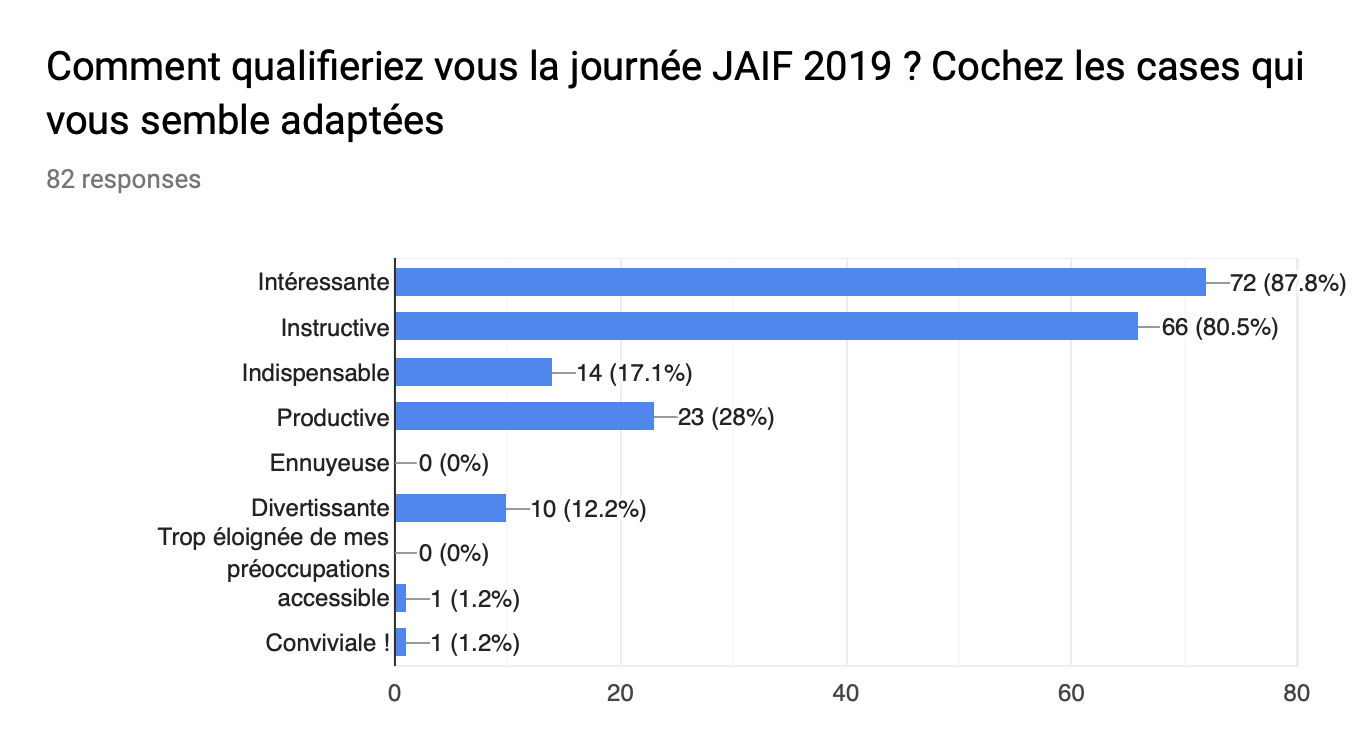
\includegraphics[width=0.65\textwidth]{images/retour_qualificatif_jaif2019.png}
\caption{Retour global sur JAIF 2019.}
\end{figure}

\begin{figure}[h]
\centering
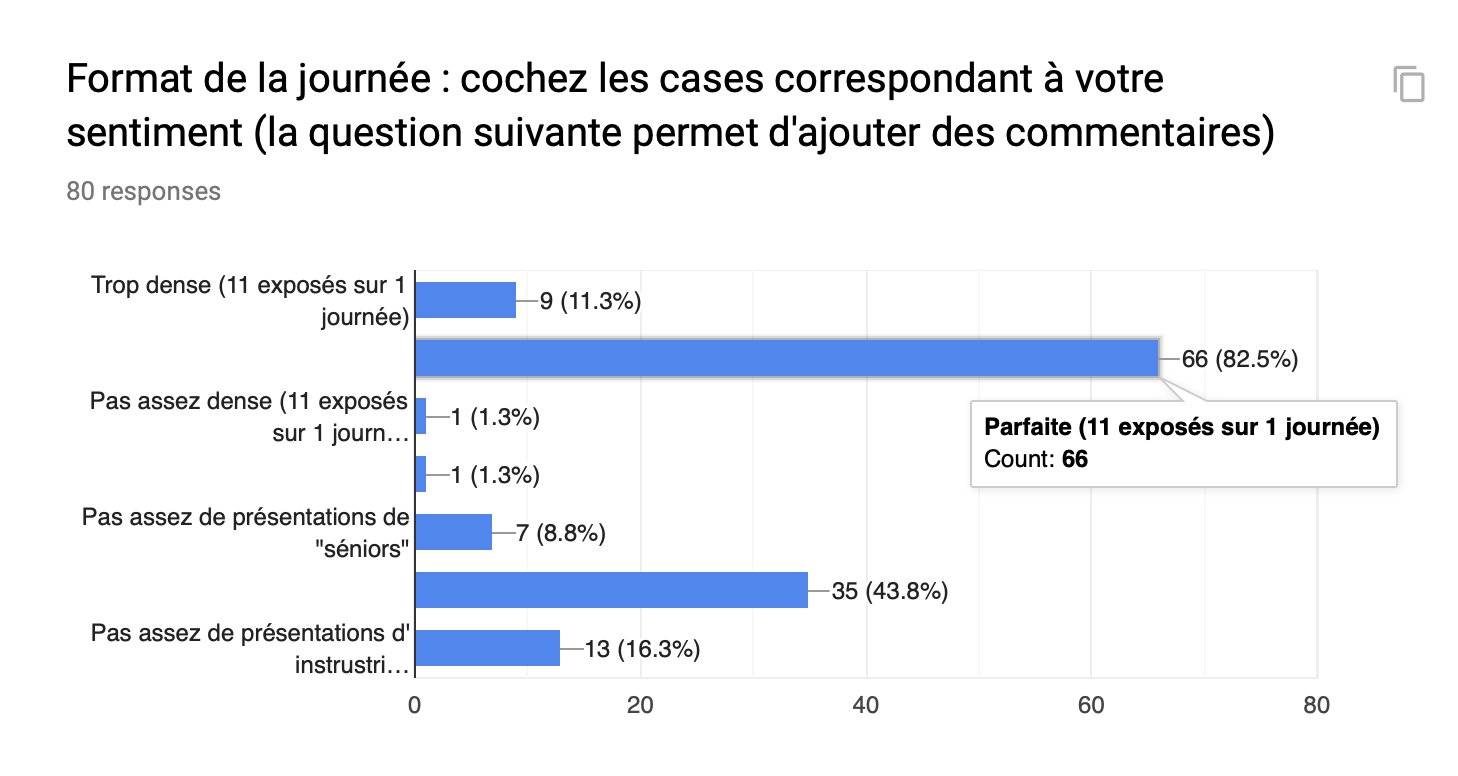
\includegraphics[width=0.65\textwidth]{images/retour_format_jaif2019.png}
\caption{Retour sur la format de JAIF 2019.}
\end{figure}

\begin{figure}[h]
\centering
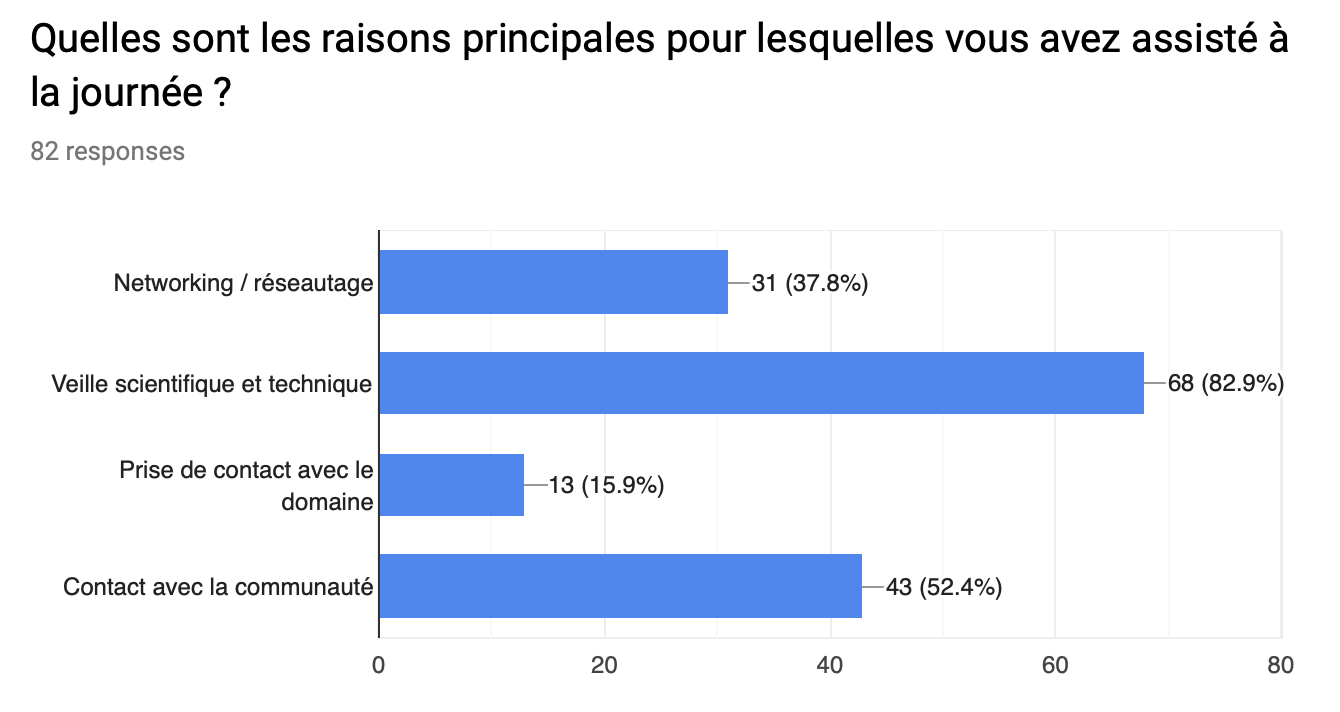
\includegraphics[width=0.65\textwidth]{images/motivations_jaif2019.png}
\caption{Motivations pour la participation à JAIF 2019.}
\end{figure}

\begin{figure}[h]
\centering
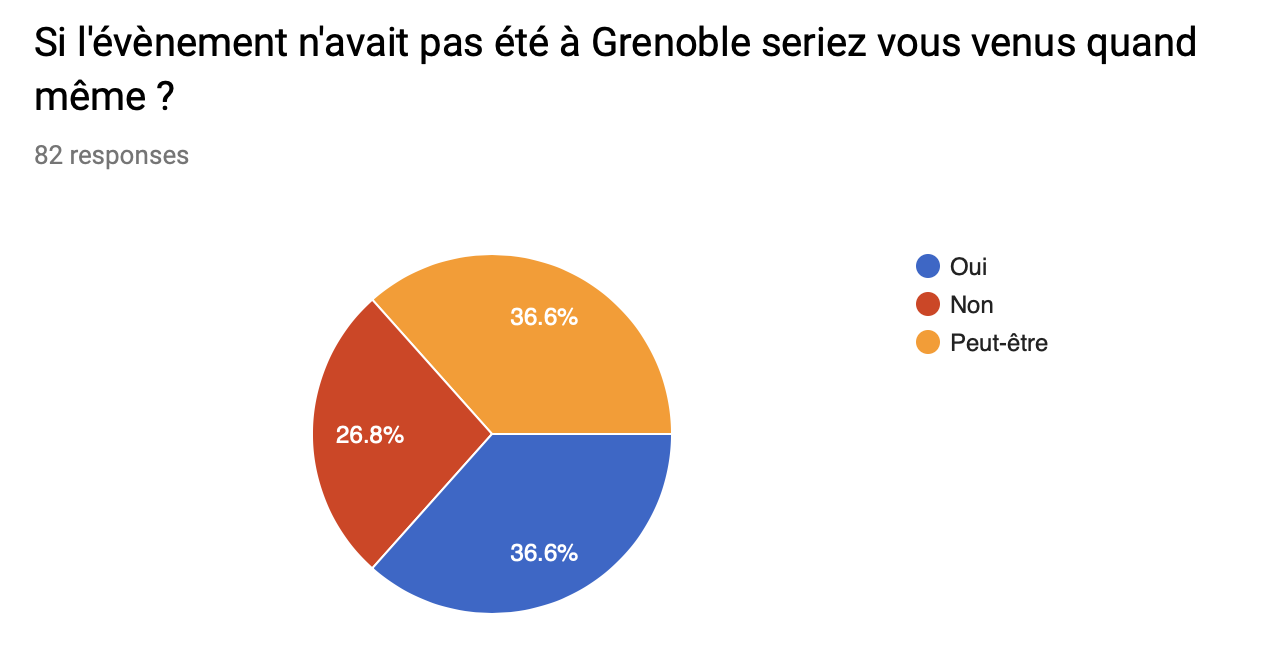
\includegraphics[width=0.65\textwidth]{images/localisation_jaif2019.png}
\caption{Impact du lieu de JAIF 2019 sur la participation.}
\end{figure}

\begin{figure}[h]
\centering
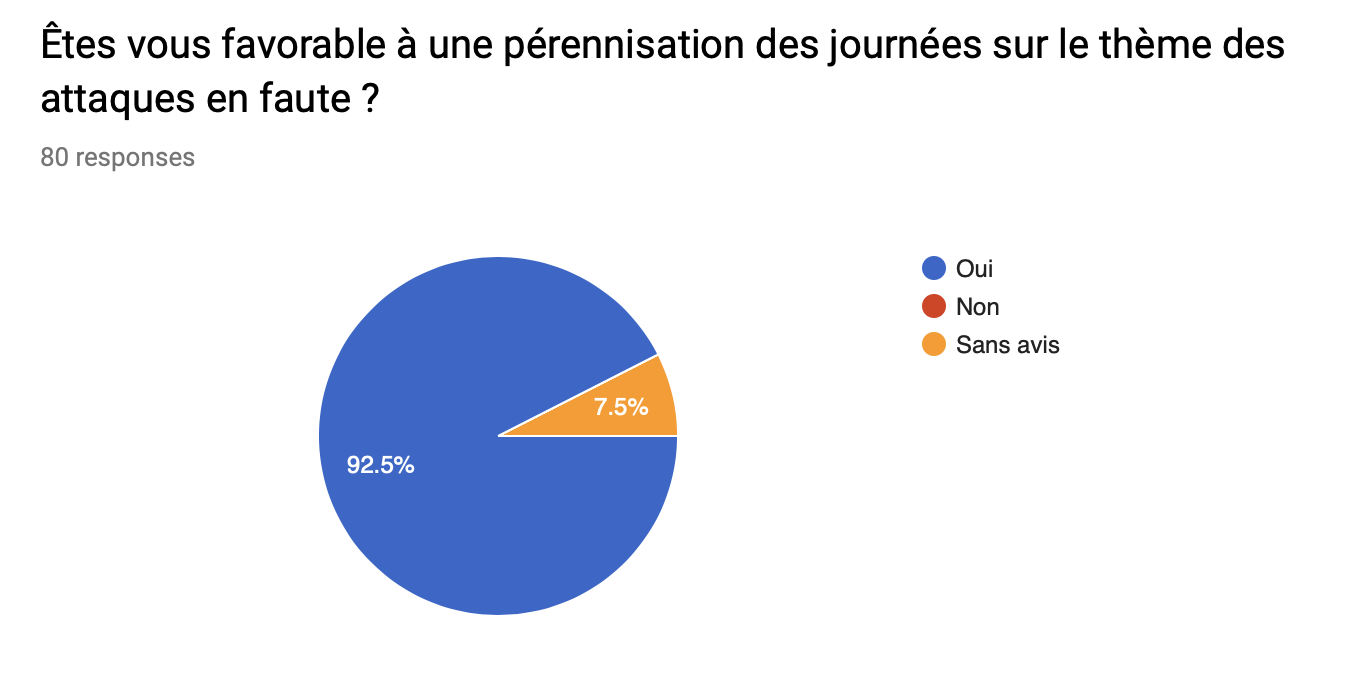
\includegraphics[width=0.65\textwidth]{images/perennisation.png}
\caption{Avis sur une pérennisation des JAIF.}
\end{figure}

\begin{figure}[h]
\centering
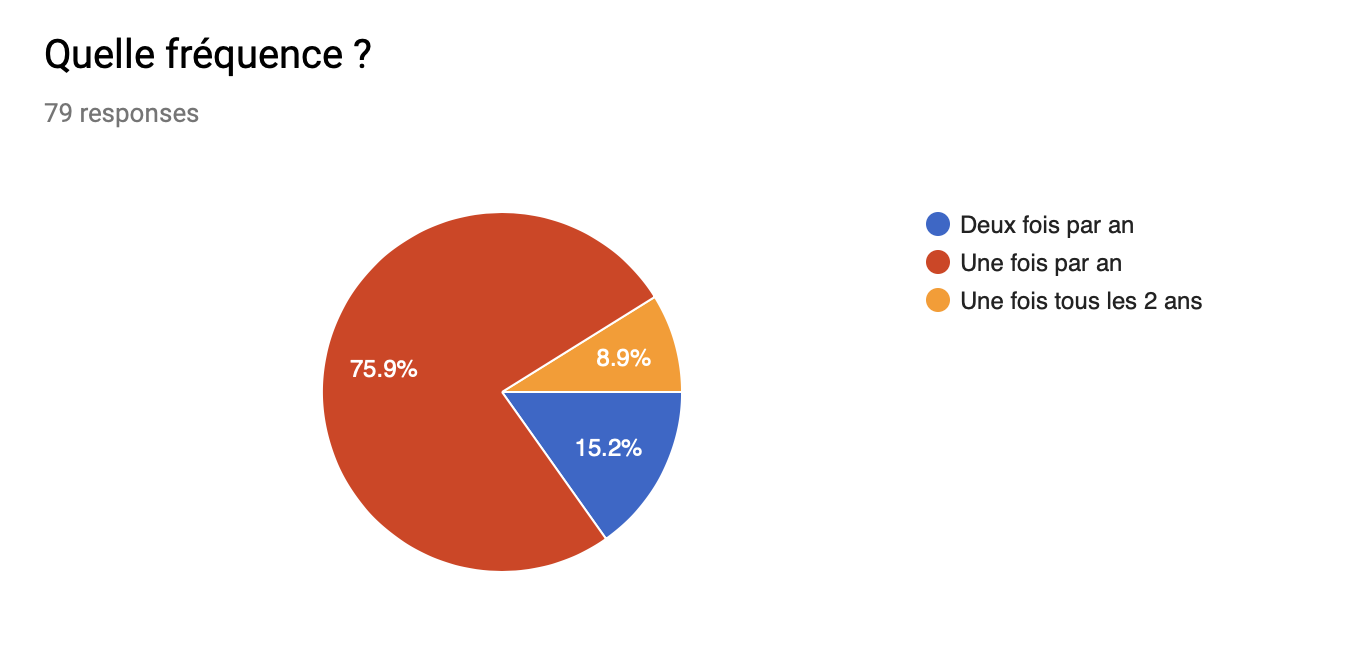
\includegraphics[width=0.65\textwidth]{images/frequence.png}
\caption{Avis sur la fréquence de futures éditions.}
\end{figure}

\begin{figure}[h]
\centering
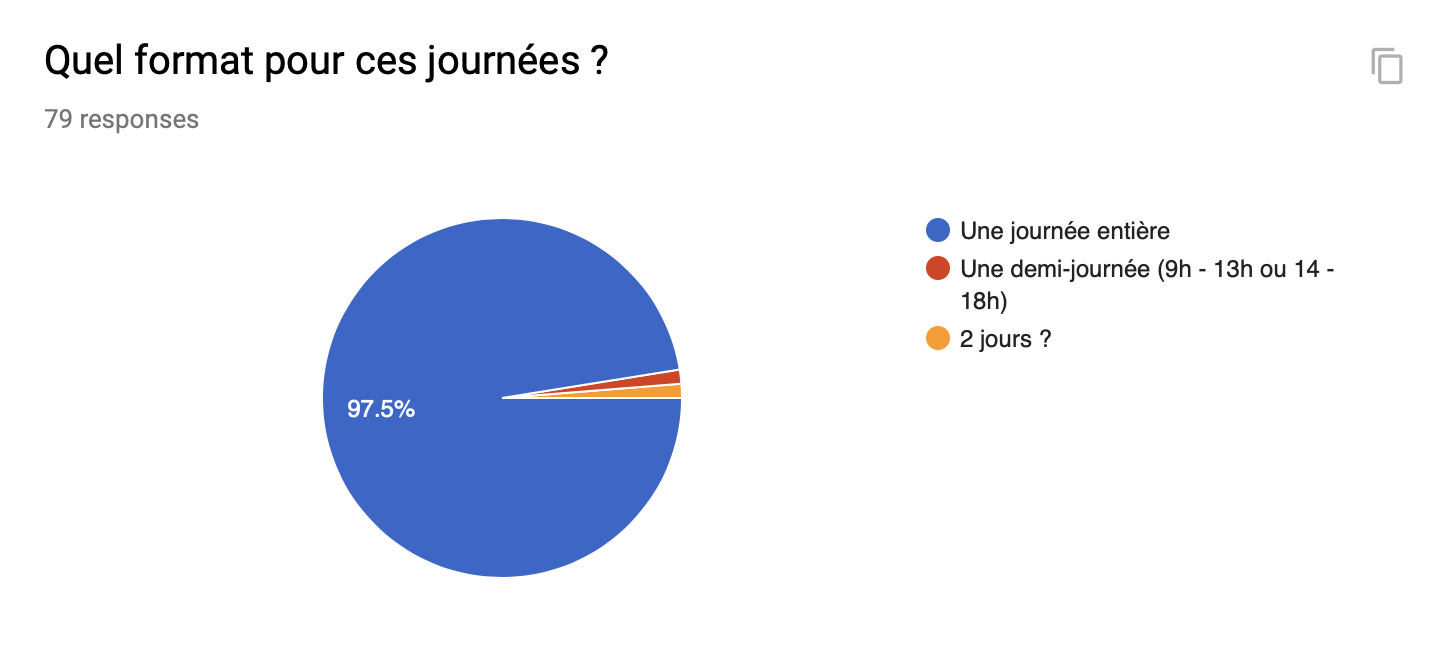
\includegraphics[width=0.65\textwidth]{images/format.png}
\caption{Avis sur le format pour de futures éditions.}
\end{figure}

\begin{figure}[h]
\centering
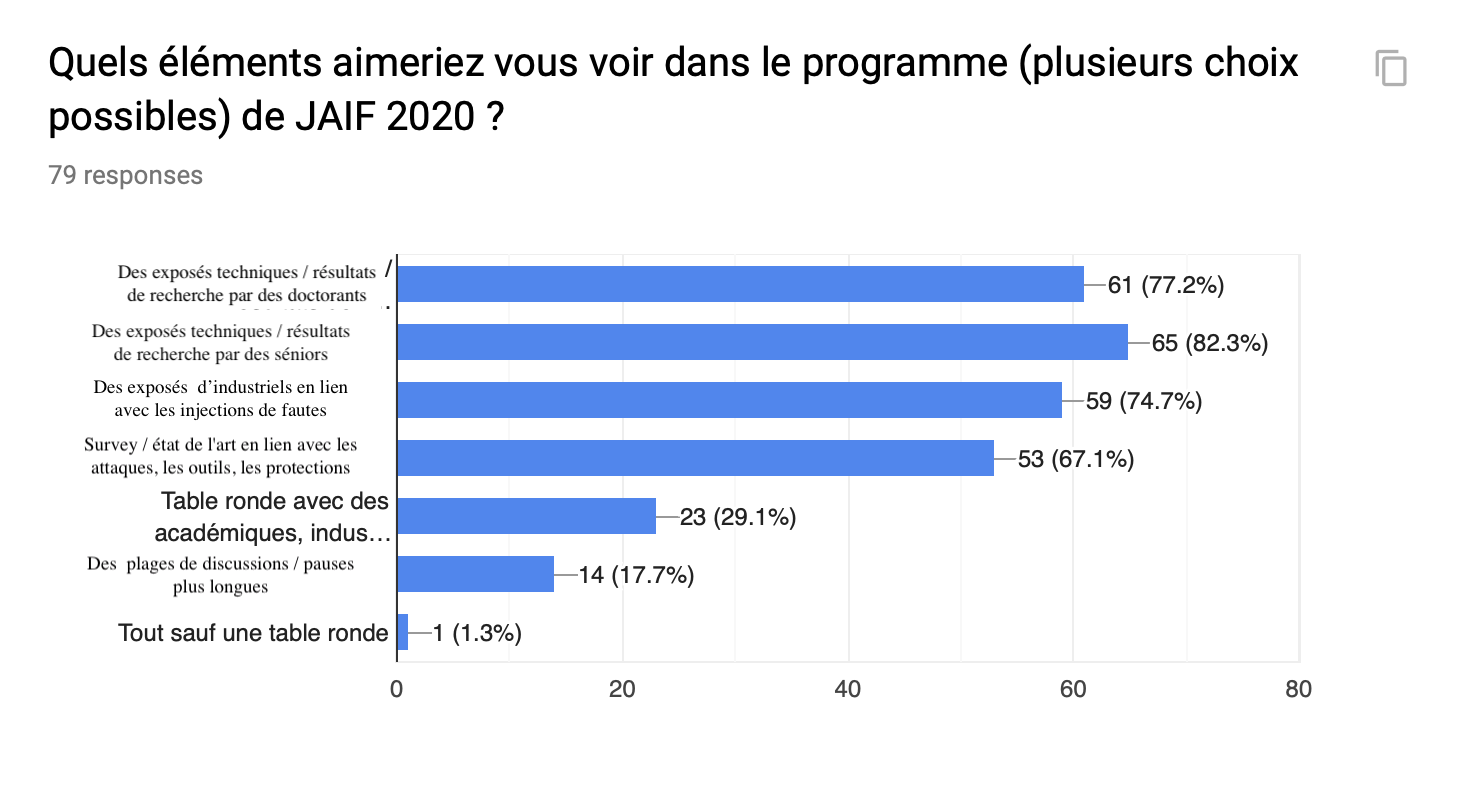
\includegraphics[width=0.65\textwidth]{images/contenu_jaif2020.png}
\caption{Avis sur le contenu pour la prochaine édition.}
\end{figure}
\end{document}
